%----------------------------------------------------------------------------------------
%	PACKAGES AND OTHER DOCUMENT CONFIGURATIONS
%----------------------------------------------------------------------------------------

\documentclass{article}
\usepackage{array}
\usepackage[english]{babel}
\usepackage[letterpaper,top=2cm,bottom=2cm,left=3cm,right=3cm,marginparwidth=1.75cm]{geometry}
\usepackage{amsmath}
\usepackage{graphicx}
\usepackage{float}
\usepackage[colorlinks=true, allcolors=blue]{hyperref}
\usepackage{todonotes}
\usepackage{setspace}
\onehalfspacing
\graphicspath{ {resources/} }

\title{Heimdall - A Kubernetes Extension}
\author{Bryan Keane}

\begin{document}

\begin{titlepage}

    \newcommand{\HRule}{\rule{\linewidth}{0.5mm}} 
    \center
    
    
    %----------------------------------------------------------------------------------------
    %	LOGO SECTION
    %----------------------------------------------------------------------------------------
    \begin{center}
        
\includegraphics{setu_logo.png}
    \end{center}
     
    %----------------------------------------------------------------------------------------
    
     
    %----------------------------------------------------------------------------------------
    %	HEADING SECTIONS
    %----------------------------------------------------------------------------------------
    \textsc{\Large Bachelor of Science (Hons) Applied Computing}\\[0.25cm]
    
    
    %----------------------------------------------------------------------------------------
    %	TITLE SECTION
    %----------------------------------------------------------------------------------------
    
    \HRule \\[0.75cm]
    { \huge \bfseries Heimdall - A Kubernetes Extension}\\[0.3cm] %document
    \HRule \\[1.0cm]
     
    %----------------------------------------------------------------------------------------
    %	AUTHOR SECTION
    %----------------------------------------------------------------------------------------
    
    \begin{minipage}{0.4\textwidth}
    \begin{flushleft} \large
    \emph{Author:}\\
    Bryan Keane 
    \end{flushleft}
    \end{minipage}
    ~
    \begin{minipage}{0.4\textwidth}
    \begin{flushright} \large
    \emph{Supervisor:} \\
    Lucy White
    \end{flushright}
    \end{minipage}\\[2cm]
    
\end{titlepage}

\newpage

\tableofcontents
\newpage

\listoffigures
\newpage

\listoftables
\newpage



\section{Plagiarism Declaration}
I declare that this material, which I now submit for assessment, is entirely my own work and has not been taken from the work of others, save and to the extent that such work has been cited and acknowledged within the text of my work. I understand that plagiarism, collusion, and copying are grave and severe offences in the university and accept the penalties that would be imposed should I engage in plagiarism, collusion or copying. I have read and understood the Assignment Regulations. I have identified and included the source of all other facts, ideas, opinions, and viewpoints in the assignment references. Direct quotations from books, journal articles, internet sources, module text, or any other source are acknowledged and the source cited are identified in the bibliography. This assignment, or any part of it, has not been previously submitted by me or any other person for assessment on this or any other course of study.  



\newpage
\section{Acknowledgements}
I would like to express my deepest appreciation to my Mentors Ciaran Roche and Laura Fitzgerald who provided invaluable experience and contributions to this project. I would also like to extend my deepest gratitude to my Project Supervisor Lucy white for guiding and encouraging me throughout the process.



\newpage
\section{Introduction}
This project, Heimdall, is an open-source Kubernetes Extension built for multi-operator Kubernetes environments. Implementing Heimdall will allow developers to configure it to watch resources of their choosing in a Kubernetes cluster. Heimdall will prevent any unwanted Operators from changing that resource, while simultaneously sending an interactive notification to the developer via a pre-configured Slack Channel regarding the issue. 



\subsection{Background}
In 2022 I completed an 8-month internship at Red Hat for my 3rd-year work placement. I worked on the Red Hat OpenShift API Management (RHOAM) team. RHOAM utilises multiple OpenShift Operators, which are automatically managed and configured applications, to provide a comprehensive API solution to its customers. The API management features provided by RHOAM include: \cite{rhoam-overview}
\begin{itemize}
    \itemsep0em 
    \item Limiting the number of API requests based on the customer’s quota
    \item Creating security policies to manage API access
    \item Monitoring API health
    \item An API portal for sign-up and documentation
\end{itemize}
While working on this team, I had the opportunity to contribute to applications which utilize various technologies like Kubernetes, OpenShift, and Go Operators.



\subsection{Motivation} 
Throughout my internship, I ran into a number of technical issues. One such issue centred around RHOAM's rate-limiting service which has become the motivation for my final year project, Heimdall. The issue in question was with the port through which API requests were being sent in order to be rate limited. That port was being overwritten by a conflicting Operator who had a different desired state for that resource. Rate limiting in this context refers to the maximum number of API calls allowed during a specified time period \cite{understanding-apis} \\\par RHOAM uses the Marin3r Operator to provide rate-limiting for RHOAM customers. It works by injecting a rate-limiting container into a Pod. The container then acts as a middleman for API requests by only redirecting requests to the destination container if the API request limit has not been reached. A more detailed explanation of this process will be discussed in \hyperlink{technologies}{Section \ref{technologies}}. \\\par It took several days of debugging to figure out what was going wrong and another week passed before my fix was merged. This meant that this problem had been occurring on customer clusters before my fix was rolled out to production. After speaking to developers on various Red Hat teams, it became apparent that this problem was not unique to our team and in fact, was an issue that all Kubernetes and OpenShift product teams face. Fixing this will not only benefit Red Hat teams but any team working on a Kubernetes-based application that utilizes Operators.


\newpage
\subsection{Problem Statement} \label{problem-statement}
In Kubernetes (K8s), resources (or objects) have a desired state which describes what the actual state of that resource should look like. The desired state can either lie in a YAML definition or in the code of a Controller. Operators and Controllers can watch that resource's actual state and continuously compare it with the desired state. If they do not match then it is the job of that Operator or Controller to make the necessary changes in order to synchronise them \cite{operator-pattern}.

\begin{figure}[H]
    \hypertarget{problem-model}
    \centering
    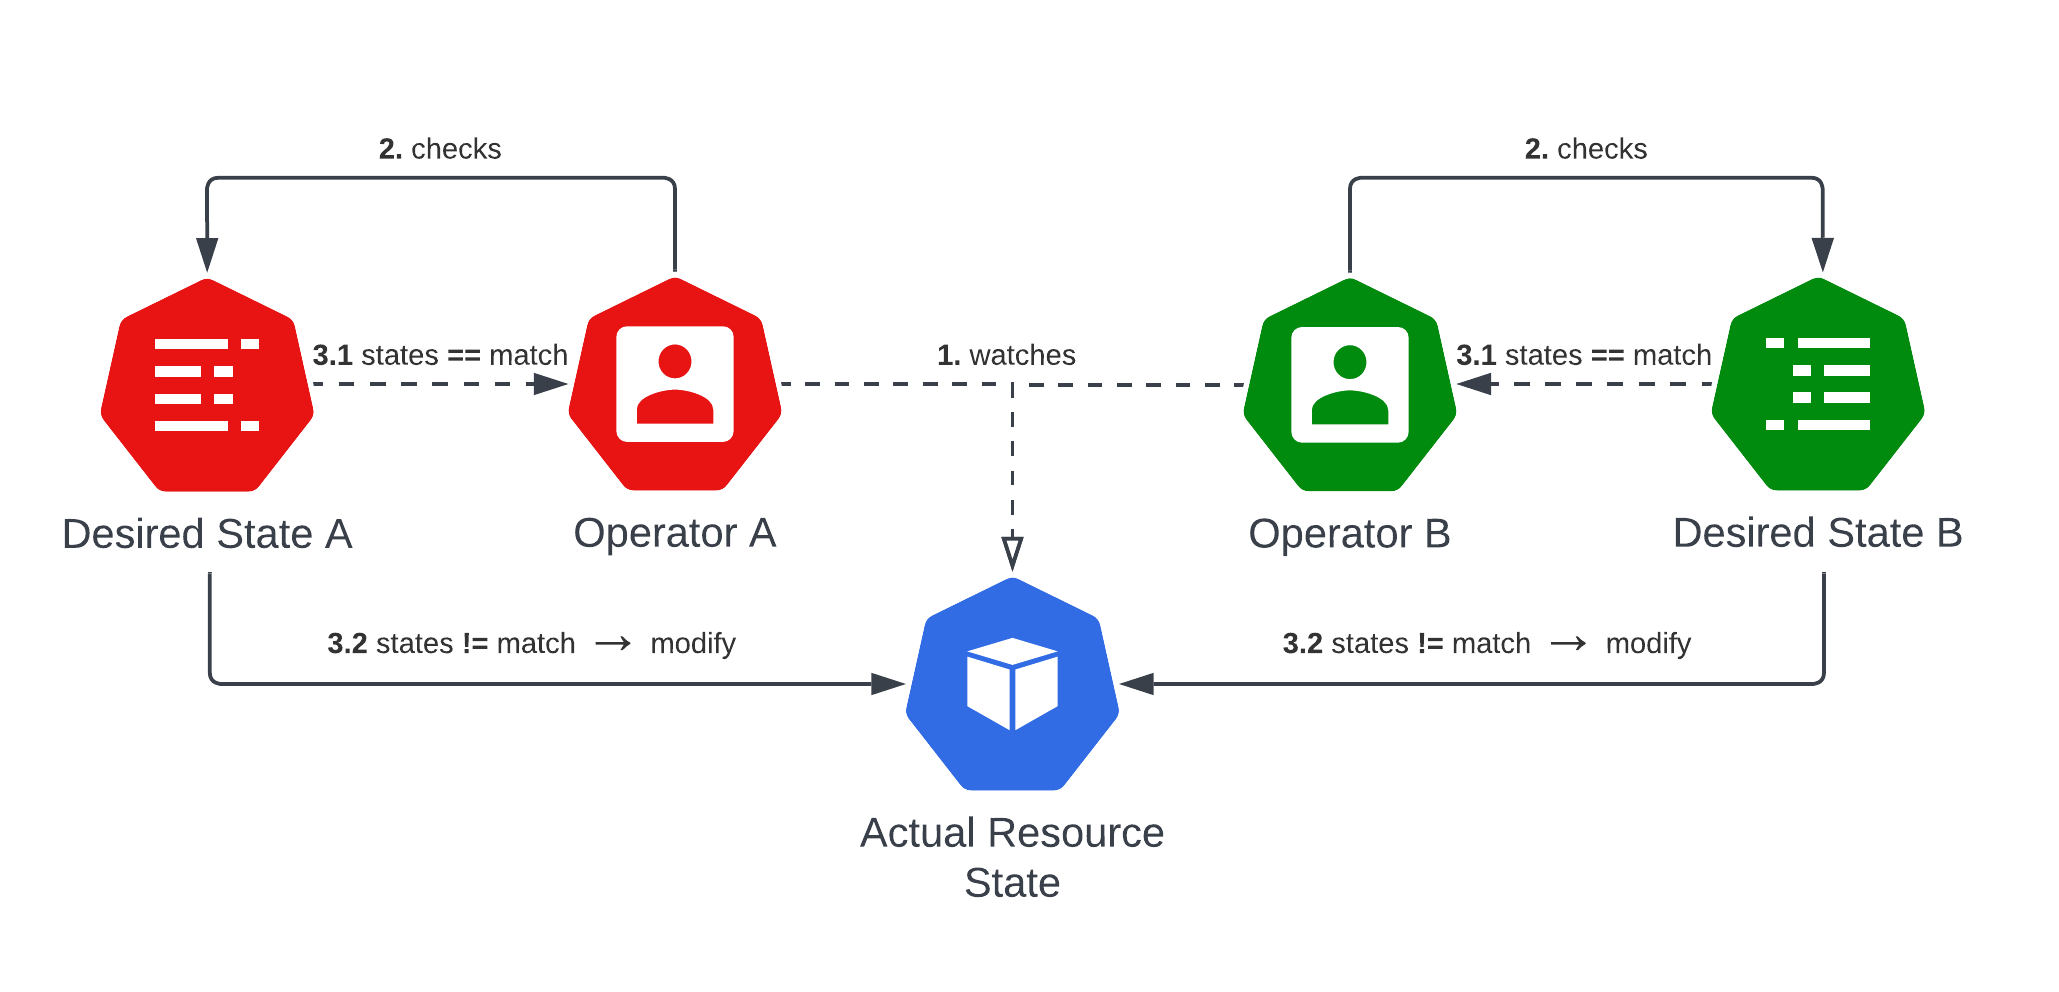
\includegraphics[width=150mm]{intro/problem-model.png}
    \caption{\emph{Model of The Problem - Two Operators Fighting Over a Resource's State}}
    \label{problem-model}
\end{figure}

This pattern works well until two Operators with conflicting desired states are both set to reconcile a resource. This will cause the resource's state to continuously change as both Operators attempt to synchronise its actual state with their unique desired state. The model shown in \hyperlink{problem-model}{Figure \ref{problem-model}} shows this problem in action. Each Operator will do the following:
\begin{enumerate}
    \itemsep0em 
    \item Watch a resource's actual state.
    \item Check the desired state for that resource.
    \item Compare the actual state with the desired state and
    \subitem 3.1. \emph{If they match} then return to Step 1. and repeat.
    \subitem 3.2. \emph{If they don't match} then modify the resource's actual state.
    \item Repeat this process continuously.
\end{enumerate}



\subsubsection{Industry Example}
As an example, the open-source e-learning platform Moodle can be used. In an educational environment, one might have a Moodle Operator and a MySQL Operator to serve as Moodle's database. The MySQL Operator manages the storing, of course, student, and module information. This application may then install a Tutors Operator, which is another e-learning platform which houses course notes and lab work. Since there is already a MySQL database via the MySQL Operator, Tutors can use the same database to store course notes and lab work. 

\begin{figure}[H]
    \hypertarget{moodle-tutors}
    \centering
    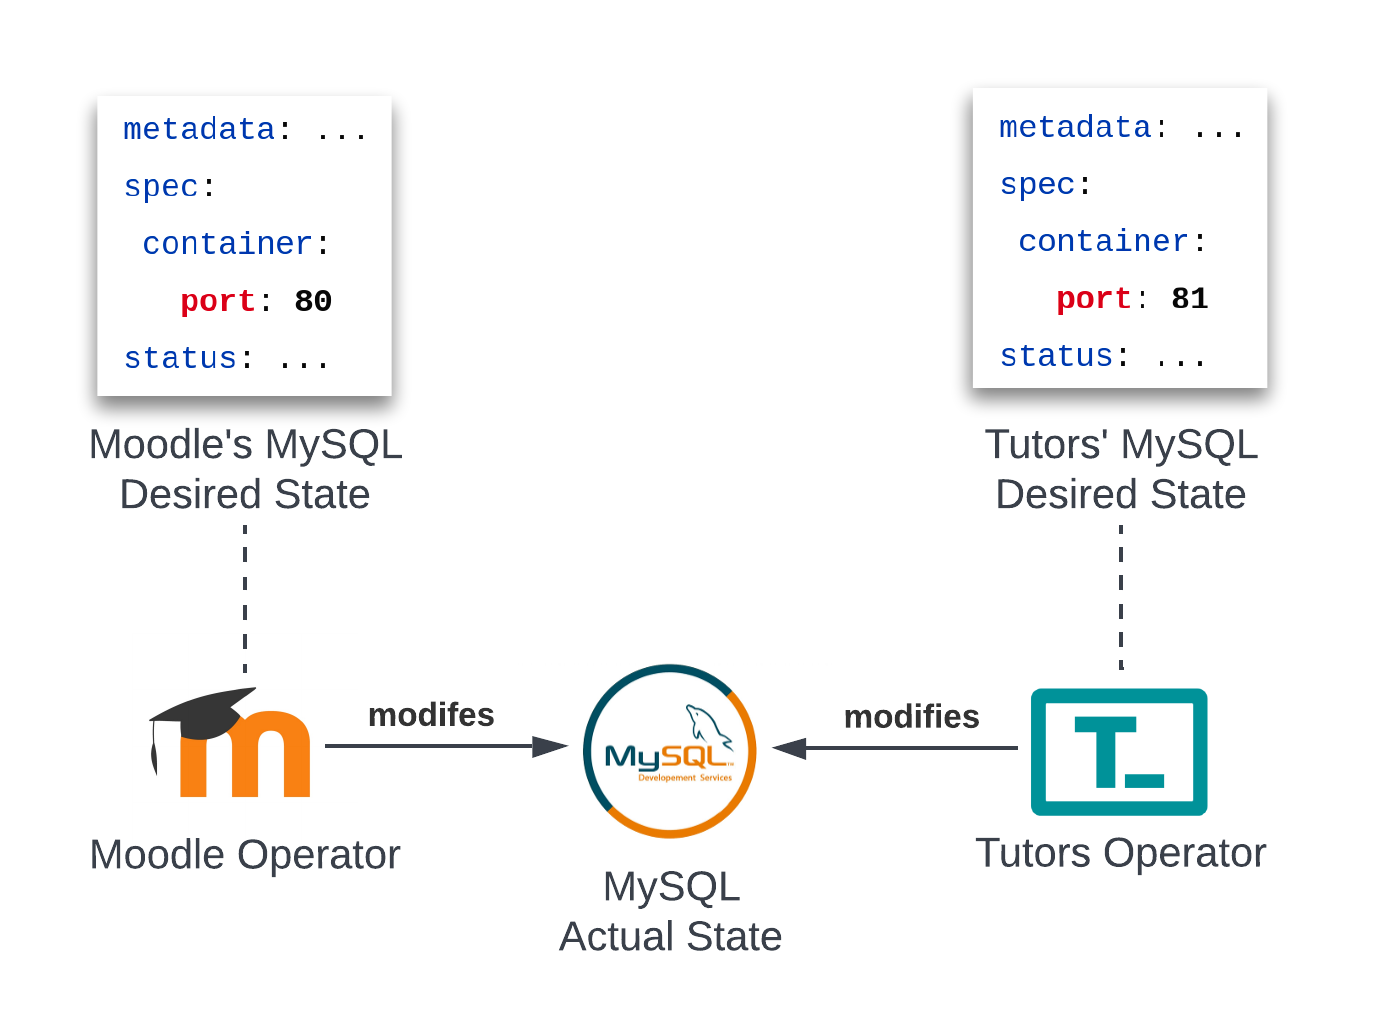
\includegraphics[width=125mm]{new-moodle-example.png}
    \caption{\emph{Simplified Model of Moodle, Tutors, and MySQL Industry Example}}
    \label{moodle-tutors}
\end{figure}

In this example, it would be very easy to misconfigure one of the Operators to have a dissimilar desired state for the MySQL resource. This would cause both Operators to constantly change that resource. Imagine Moodle wanted the port in which database access occurred to be port 80 and Tutors wanted the database access to occur through port 81. This would cause the MySQL resource's access port to be changed back and forth. If a lecturer or student attempts to access information through Moodle, but at that point in time the MySQL resource's port was configured by the Tutors Operator, the user would not be able to retrieve the data. 

\subsection{Aims and Objectives}
The solution is to create a custom Kubernetes controller which will monitor resource states. A Kubernetes Operator can create a resource, become its owner, and will set the controller to watch that resource for changes. If another operator changes the resource the controller will trigger an alert, notify the developer via a slack integration and allow the developer to fix the problem without the need for time-consuming debugging. 

\begin{figure}[H]
    \hypertarget{solution-model}
    \centering
    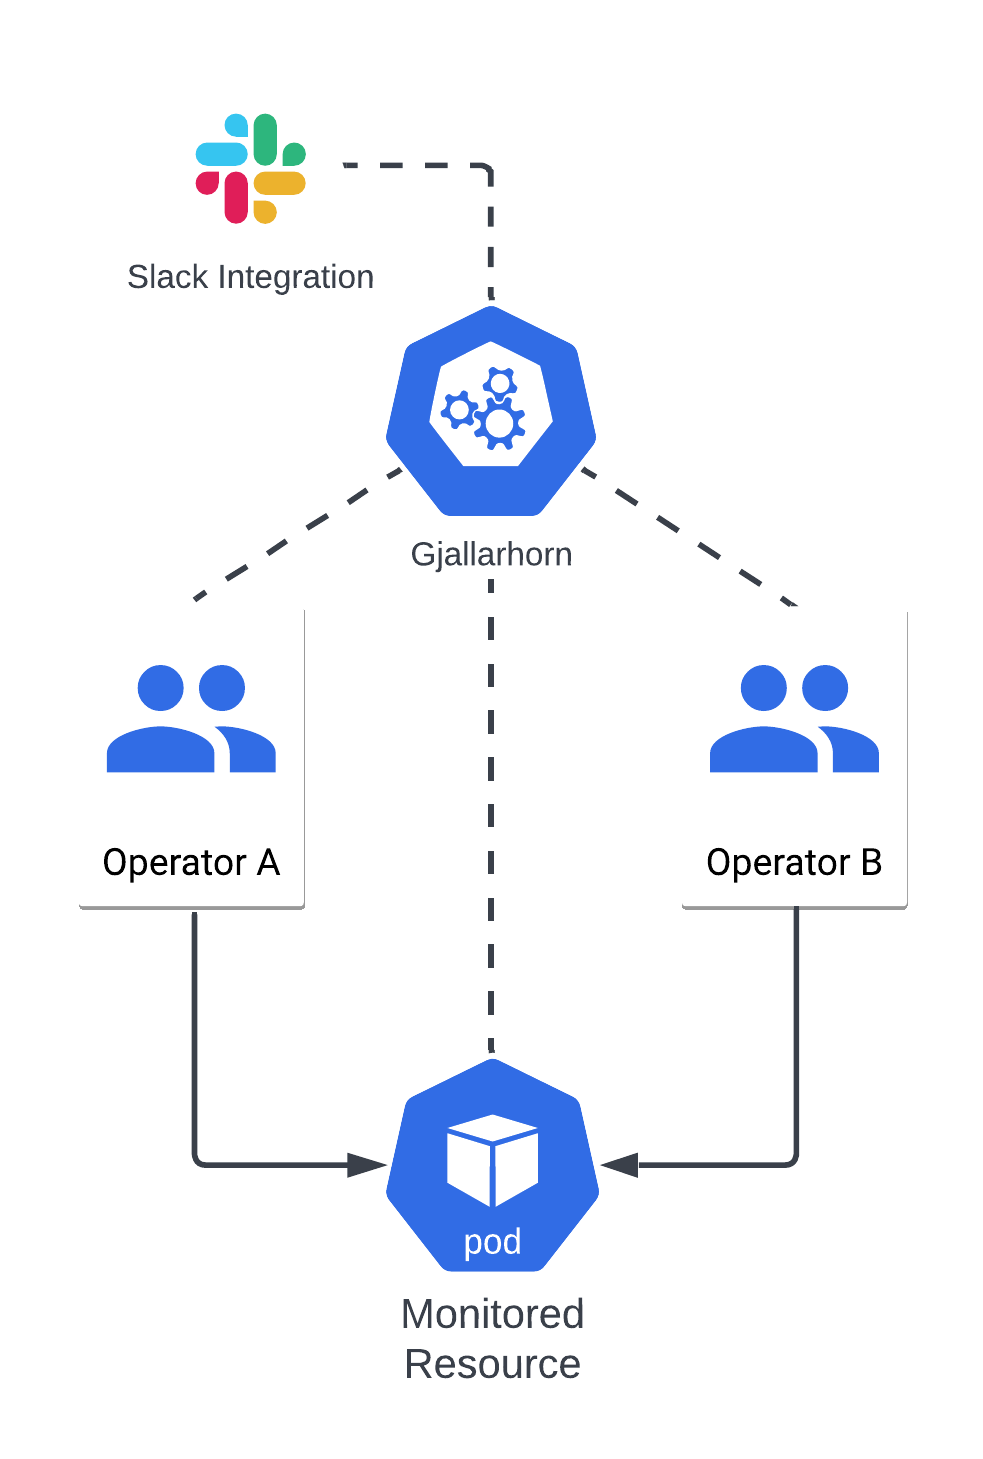
\includegraphics[width=100mm]{solution-model.png}
    \caption{\emph{Model of the solution: Heimdall}}
    \label{solution-model}
\end{figure}

\hyperlink{solution-model}{Figure \ref{solution-model}} models the proposed solution where the Owner Operator and Rogue Operator are attempting to change a resource's actual state. Once the Owner Operator is installed, it creates the resource with the addition of a label that Heimdall is looking for. Heimdall sees a new resource created with this label and begins monitoring its state. The Rogue Operator is installed and begins changing the resource. \\\par The minimum viable product for Heimdall involves the controller watching for non-owners changing the state of a resource. It will then generate an interactive notification for slack with details on the issue to allow the developers to find and fix the problem with relative ease. The stretch goals for Heimdall will involve allowing for an atomic owner of a resource to be set and blocking changes from non-owners. This will not only allow the developer to fix the problem with ease but also stop the issue from occurring and prevent any downtime for the end user. These will be discussed further in Section \ref{stretch-g}. 



\subsection{Risk Analysis}

Various risks are associated with the implementation of Heimdall, one of which is far more significant than the others. During the initial research into the viability of this project, there were no examples or previous attempts found that try to implement such a solution. This poses a significant risk as it means that it is not guaranteed that the implementation will be technically possible. An appropriate risk mitigation strategy is needed in order to ensure that the creation of Heimdall can still be completed to some degree. To do this, the project has been split up into a Minimum Viable Product (MVP) and stretch goals which are discussed further in Sections \ref{mvp} and \ref{stretch-g}. If after exhausting all attempts to implement the stretch goals, it is found that it is not possible, the MVP still provides a valid solution to the problem. \\\par If the implementation is confirmed to be technically possible, the next risk will be that the project cannot be completed within the given time constraint. Again, this can be partially mitigated by the use of the MVP and stretch goals. Although, with the use of the chosen methodologies discussed in Section \ref{methodology}, the use of Sprints and following a Continuous Delivery approach to development should mitigate any concerns about time.

\subsection{Outline}
With the motivation, problem, and proposed solution discussed, a more in-depth discussion of some low-level components is necessary to understand the inter-workings of how Heimdall will operate.

 
\section{Methodology} \label{methodology}
The chosen methodology for software development teams is paramount for the successful planning and development of a product. Historically, the Waterfall Methodology was commonplace - but now Agile is the gold standard. Waterfall involved a distinct sequence of actions for engineers to follow. In short, it involved extensive design and planning before ever writing a line of code. Long documents detailing product design and strategy were written to fit the stakeholder's requirements. This proved to be ineffective as in most cases, holes in the design are discovered after beginning the implementation. In recent years, Agile has begun replacing this framework as it has proven much more efficient for software development teams \cite{agile-waterfall}.



\subsection{Agile}
"Agile is an iterative approach to project management and software development that helps teams deliver value to their customers faster and with fewer headaches" \cite{what-is-agile}. 



\subsection{Scrum Roles}
Scrum has three main roles: Scrum Master, the Product Owner, and the Development Team. These are used to help describe the responsibilities of each stakeholder for a product.



\subsection{Scrum Artifacts}
Teams who practice Agile and Scrum methodologies often collect Scrum Artifacts. These are pieces of information that a product's stakeholders and the team developing it use to describe its development. The main Scrum Artifacts used for this project include Product Backlog Refinement, Sprint Planning, and Sprint Reviews. There are also various Extended Artifacts that are not included in the official Scrum Artifacts definition. These include reporting mechanisms like Burn down Charts.



\subsection{Version Control}
What is VCS, Git, GitHub 



\subsection{Continuous Integration}
Version control lies at the heart of Continuous Integration. CI is an Agile practice of integrating code changes to a product automatically from various contributors (product teams and open-source community contributions). It is a method used to consistently merge code changes into one central repository which runs automated tests and builds to ensure code functionality and integrity.   



\subsection{Continuous Delivery}
Continuous Delivery is an approach 



\subsection{Testing Approach}



\subsection{Open Source}



\section{Technologies} \label{technologies} 



\subsection{Kubernetes}

Kubernetes is an open-source tool used to implement modern micro-service-based architectures. It can be used to create, manage, and deploy containerized applications and is commonly known as a container orchestrator \cite{k8s-overview}. Containers are small processing units which house applications and their dependencies. They are bundled up into a singular image that is able to run on any hardware. This removes the need for installing required packages when attempting to run an application. Kubernetes orchestrates the deployment of many containers to form larger applications that are highly available, fault-tolerant, and have high degrees of redundancy.



\subsubsection{Resources} \label{resources}

Resources, also known as objects, are how the state of a Kubernetes cluster is represented. These resources are detailed in \emph{.yaml} format \cite{k8s-obj}. They usually describe the following key pieces of information:

\begin{itemize}
    \itemsep0em 
    \item Which container image is being used
    \item The compute resource available to the application, namely CPU and Memory limits
    \item Resource policies on how things like fault tolerance, upgrade behaviour, and restart behaviour should operate
    \item General resource information like the Namespace, Labels, and Annotations
\end{itemize}

The lowest-level Kubernetes resource is a Pod. Pods house the containers that run applications. They are expendable and can never be edited. If the desired state of a Pod is changed, it is destroyed and recreated to match the Pod's actual state with the new desired state. This also increases the cluster's degree of fault tolerance as if one Pod fails, instead of trying to recover it the Pod can be deleted and redeployed. 

\begin{figure}[H]
    \centering
    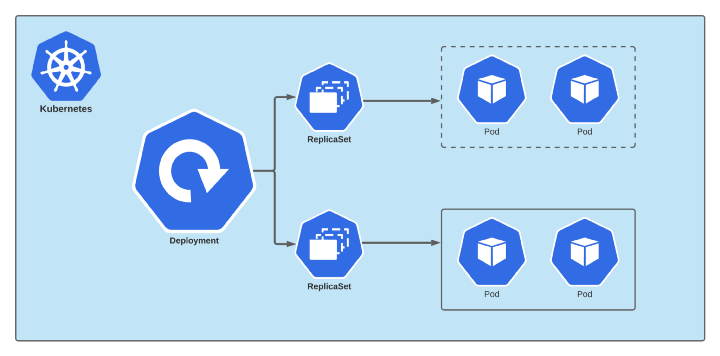
\includegraphics[width=160mm]{tech/resource-struct.png}
    \caption{\emph{Kubernetes application Resources: Deployments, Replica Sets, and Pods}}
    \label{resource-struct}
\end{figure}

There are two other Resources which make up the structure of a running application in Kubernetes. Figure \ref{resource-struct} \cite{k8s-rolling} details how Deployments and Replica Sets work with Pods in order to complete an application's workflow. Deployments are the top-level Resources in this structure and typically act as the source of truth (desired state) for Pods. If a Deployment's \emph{.yaml} specification is changed by another Controller, then its Pod's desired state will change and be redeployed. The Deployment also acts as a desired state for Replica Sets, which are responsible mainly for managing the number of Pod replicas currently running. 

\begin{figure}[H]
    \centering
    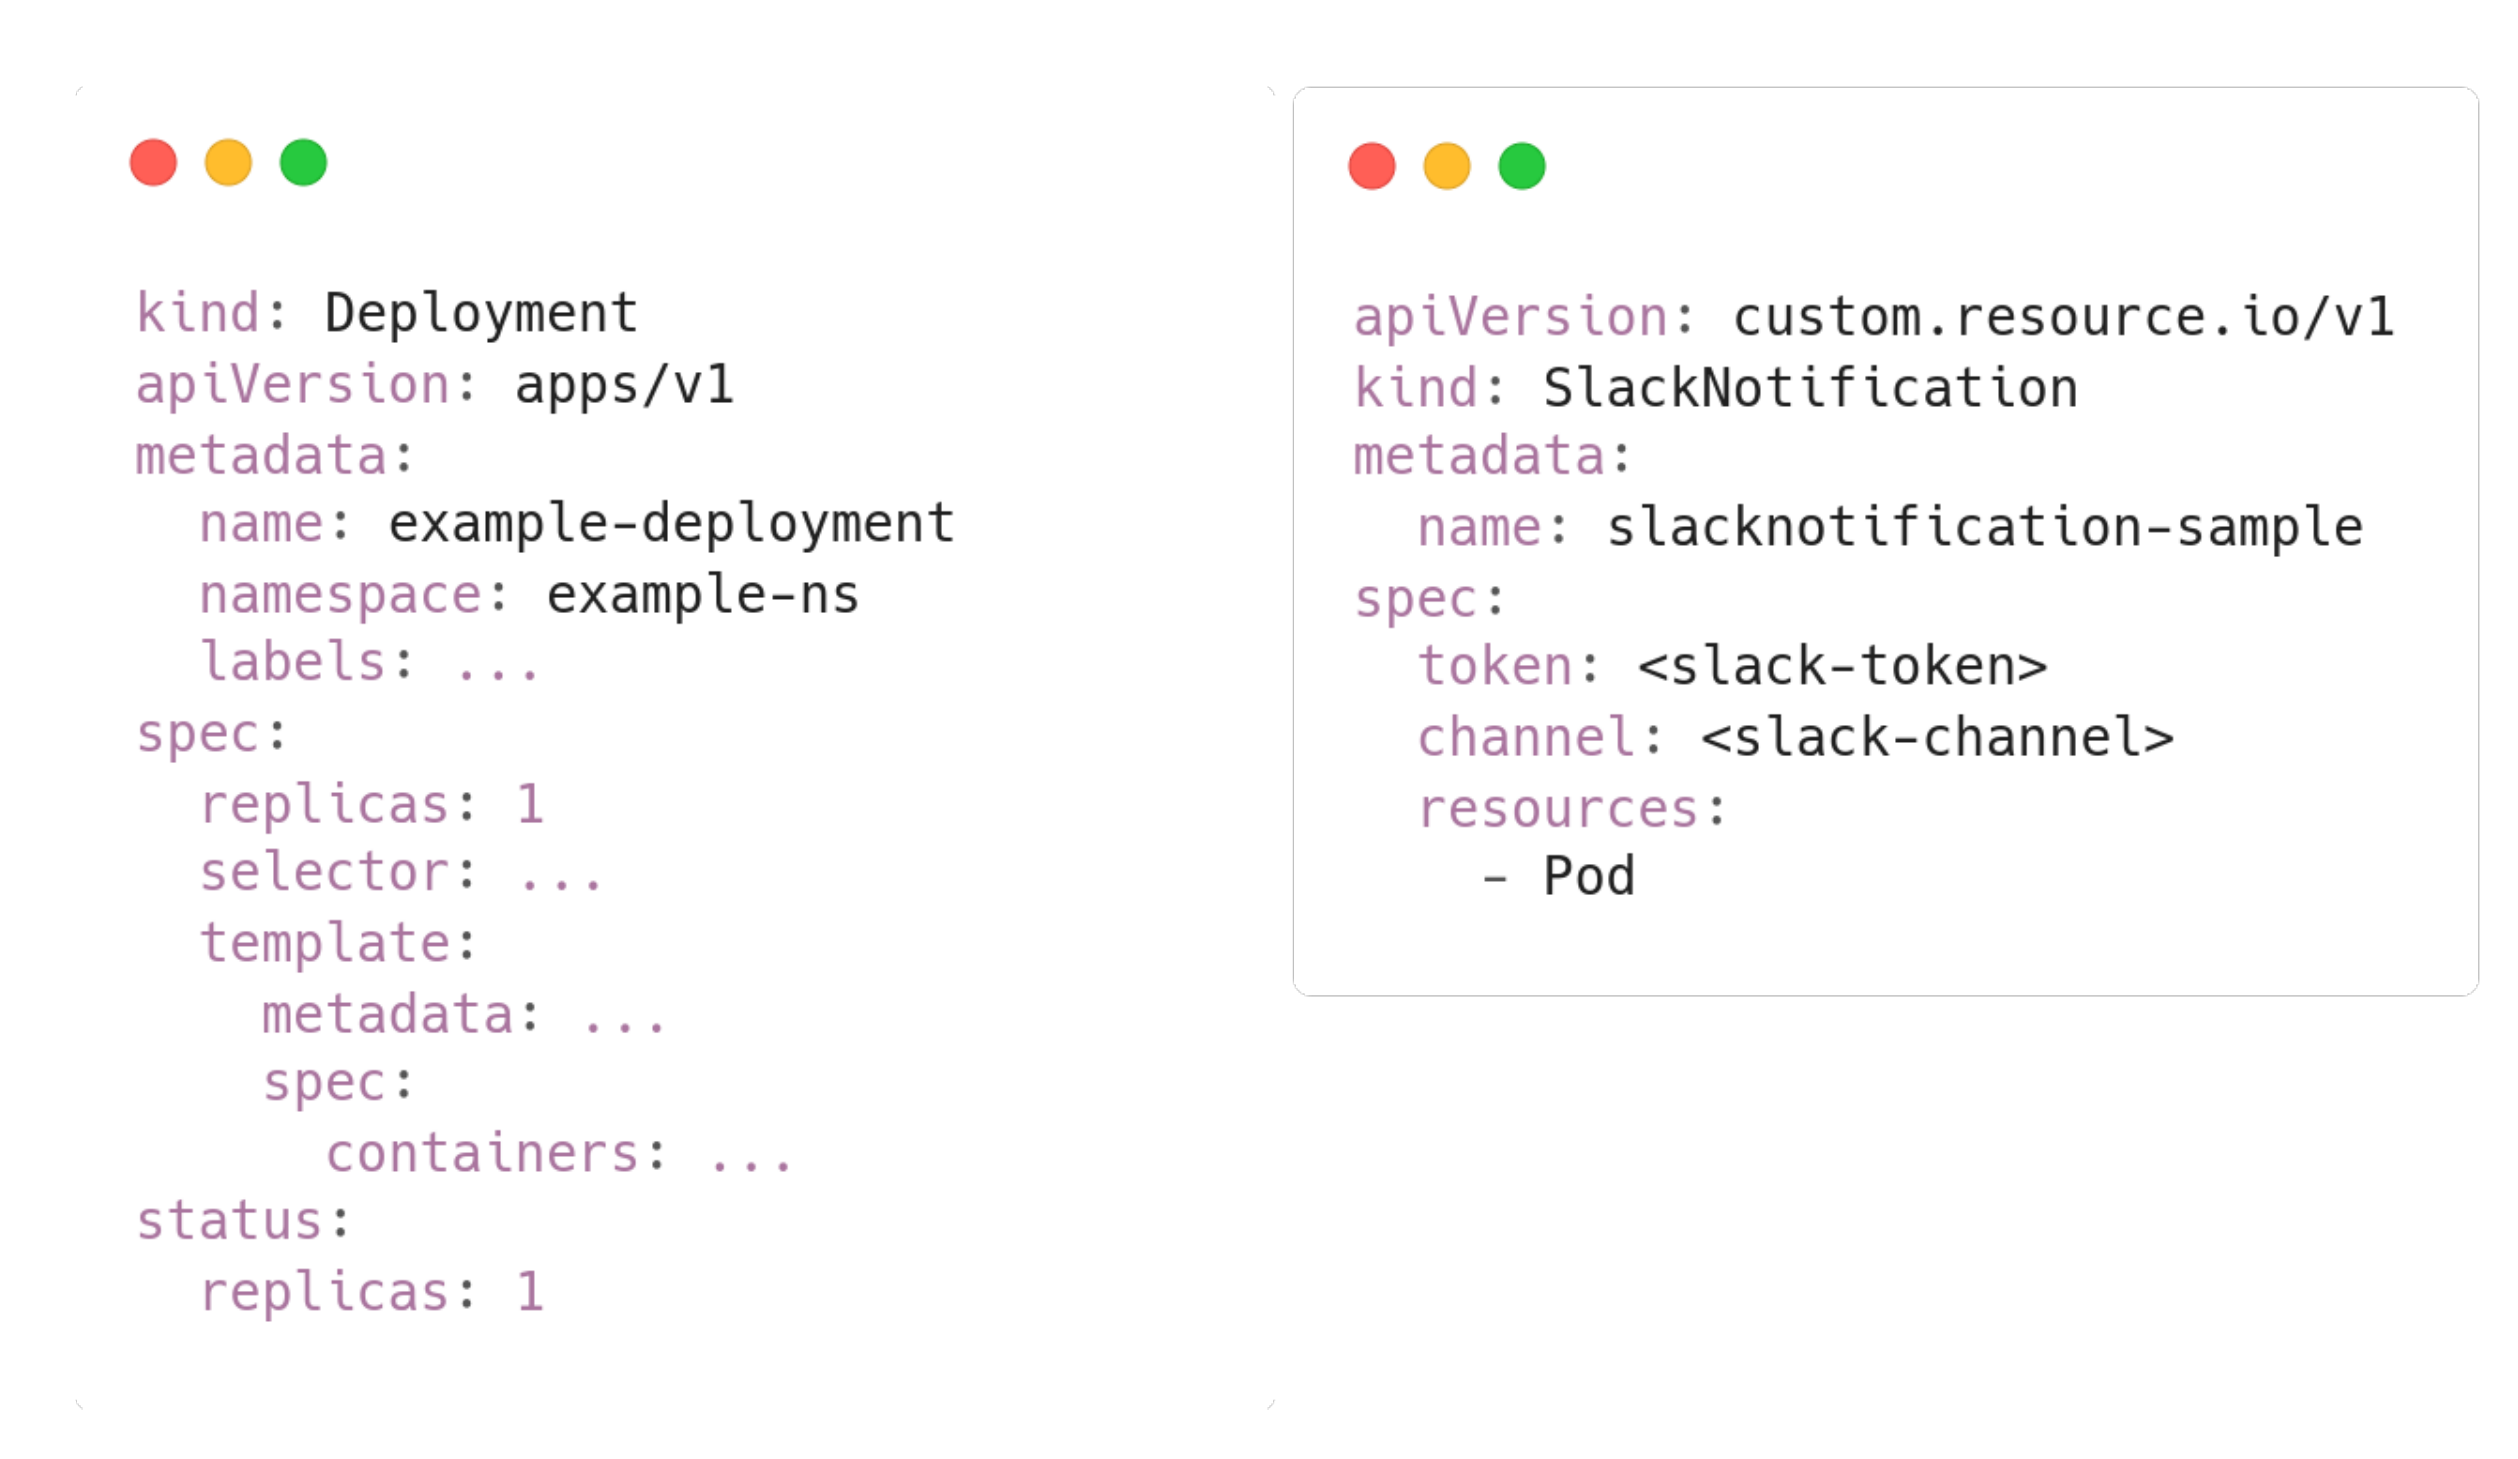
\includegraphics[width=125mm]{tech/core-cr.png}
    \caption{\emph{Example Core Resource (Deployment) comparison with Example Custom Resource}}
    \label{core-cr}
\end{figure}

Aside from core resources, there are also custom resources. They extend the Kubernetes API outside of the typically available resource types. They allow for customisation of the typical resource fields like \emph{.spec} and can be reconciled (watched and maintained) by custom controllers \cite{cust-res}. An example \emph{yaml} definition of a Deployment (Core Resource) and a Custom Resource (Slack Custom Resource Example) can be seen in Figure \ref{core-cr} As seen, the Custom Resource (on the right) can have any custom fields in the Resource's \emph{.spec} and the Kind and API Version values are different to that of Core Resources.



\subsubsection{Controllers} \label{controllers}

As already explored in Section \ref{problem-statement}, Controllers are predominately responsible for watching the actual state of resources and matching it with their desired state. An example would be the Deployment Controller which ships natively on Kubernetes clusters. It ensures that the actual state of all Pods matches their desired state described in its Deployment. Custom Controllers can also perform various different operations including interacting with services outside of a cluster, like sending notifications to a Slack Channel \cite{ctrlrs-ref}. Custom Controllers and Custom Resources packaged up together to create one application are what Kubernetes refer to as the Operator pattern.


\subsubsection{Operators}

The core purpose of Operators is to attempt to perform the actions a human operator might. This includes monitoring, managing, and maintaining an application. This is done instead through code where an Operator is installed onto a cluster and will automatically handle any failures, react to changes in the cluster, and carry out actions upon specific events occurring \cite{operator-pattern}. This could be as simple as managing a web server and scaling up the number of web server pods as it gets more traffic to prevent Pod failure.
\begin{figure}[H]
    \centering
    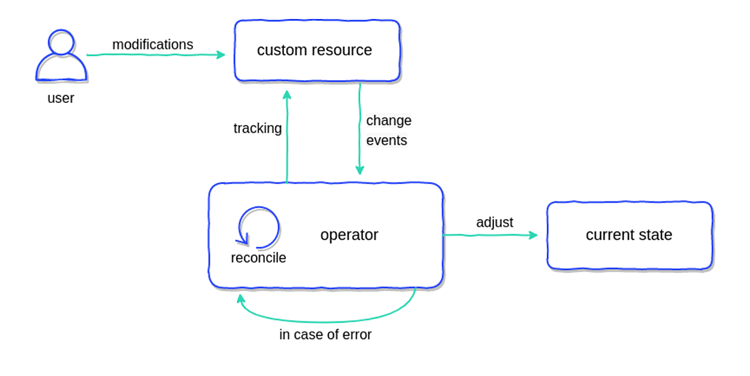
\includegraphics[width=160mm]{tech/operator-pattern.png}
    \caption{\emph{Operator Pattern model of Custom Controller and Resources interaction}}
    \label{op-pat}
\end{figure}

Whatever the use case, they serve the purpose of automating tasks beyond what Kubernetes provides out of the box. A model of the Operator pattern taken from the Container Solutions blog can be seen in Figure \ref{op-pat} \cite{op-pat-blog}. In order for Operators to carry out the tasks they need to perform, they need to be granted permission to complete them. 



\subsubsection{Role-Based Access Control}

Kubernetes environments use a Role-Based Access Control (RBAC) method to allow applications to perform certain tasks. Since the API Server acts as a mediator for all Kubernetes actions, the rules which describe a user's permissions use the verbs common to APIs like \emph{GET}, \emph{POST}, and \emph{DELETE} \cite{rbac}. First, applications (Controllers, Pods, Operators, etc) are assigned a Service Account. Roles can then be created which describes what actions any application assigned with that Role can take. Finally, Bindings can be created to link these Roles to specific Service Accounts. This method of permission granting will likely prove useful for the implementation of the Stretch Goal discussed in Section \ref{stretch-g}.




\subsubsection{Unstructured Package}

Section \ref{controllers} detailed how Controllers can watch specific resources for events. Controllers can be configured to watch Resources which contain a specific label like \emph{heimdall: watching}. This is useful as it means a Controller can watch and perform actions on any Resource which can be dynamically configured. An issue arises when we consider the Resource kind the Controller is being told to watch. If a Controller is set to watch a specific Resource, it requires a Kind to be specified, which could be \emph{Pod}, \emph{Deployment}, etc. What if the Controller is configured to only watch Pods with a specific label but then that label is added to a custom resource which does not contain the kind \emph{Pod}. This is where the Unstructured Package comes into play. This package allows for a Controller to watch and interact with Resources of any Kind. This will be integral to the implementation of Heimdall as the Controller will need to complete its task on any Resource in a cluster regardless of its Kind. This is discussed further in the final proof of concept in Section \ref{unstructured-poc}.




\subsection{Languages}
\subsubsection{GoLang}
\subsubsection{yaml}



\section{Tools}
Minikube, Operator SDK, Docker, Git, GitHub, Jira, Slack Client, Golang, GitHub Actions, Overleaf



\section{Design}



\subsection{System Architecture Overview}
Create a diagram


\subsection{Minimum Viable Product} \label{mvp}


\subsection{Stretch Goals} \label{stretch-g}



\subsection{Requirements}



\subsubsection{Functional Requirements}
What the project actually does
From a devs POV



\subsubsection{Non Functional Requirements}
Under the hood what I need to get working. Security




\subsection{User Stories}
As a Developer, I want to be aware of changes to resources that I own so that I can take action if an unwanted change is made.
As a Developer, I want to control the cadence of alerts so that I can control the noise created by those alerts.
As a Developer, I want to claim ownership of the resources that I control.
As a Developer, I want to control the changes to resources that I own.



\subsection{Personal Stories}
As a student, I want to have achieved First Class Honors, so that I can reach my academic goals.

As an aspiring Software Engineer, I want to contribute a solution to a common problem faced by Software Engineers working with Kubernetes, so that I can make a valuable contribution to the open-source community.



\subsection{User Definitions}



\subsection{Models}



\section{Proof of Concept}
There are three prototypes necessary for the planning of Heimdall. 

\subsection{Slack Prototype}

\subsection{Watcher Prototype}

\subsection{Unstructured Prototype} \label{unstructured-poc}

\section{Reflection}



\section{Summary}



\subsection{Review}



\subsection{Semester Two Outline}

\bibliographystyle{alpha}


\clearpage
\begin{thebibliography}{9}


\bibitem[What is Agile?, 2022]{what-is-agile}
\emph{Atlassian}, \\URL: https://www.atlassian.com/agile 

\bibitem[Operator Pattern, 2022]{operator-pattern}
\emph{Kubernetes}, \\URL: https://kubernetes.io/docs/concepts/extend-kubernetes/operator/

\bibitem[IBM API-Connect, 2022]{understanding-apis}
\emph{Understanding rate limits for APIs and Plans}, \\URL: https://www.ibm.com/docs/en/api-connect/10.0.1.x?topic=connect-understanding-rate-limits-apis-plans

\bibitem[M. McCormick, 2012]{agile-waterfall}
\emph{Waterfall vs Agile Methodology}, M. McCormick, \\2nd ed. MPCS, Inc., 2012.

\bibitem[I. Sommerville, 2021]{agile-book}
\emph{Engineering Software Products: An Introduction to Modern Software Engineering}, 2021.
  
\bibitem[Kubernetes Overview, 2022]{k8s-overview}
\emph{Kubernetes}, \\URL: https://kubernetes.io/docs/concepts/overview/  

\bibitem[Red Hat Developer, 2020]{rhoam-overview}
\emph{Red Hat OpenShift API Management}, Red Hat, 2020. \\URL: https://developers.redhat.com/products/red-hat-openshift-api-management/overview

\bibitem[K8s Objects, 2022]{k8s-obj}
\emph{Understanding Kubernetes Objects}, Kubernetes. \\URL: https://kubernetes.io/docs/concepts/overview/working-with-objects/kubernetes-objects/
  
\bibitem[Y. Maharjan, 2020]{k8s-rolling}
\emph{How Rolling and Rollback Deployments work in Kubernetes}, Medium, 2020. \\URL: https://yankeexe.medium.com/how-rolling-and-rollback-deployments-work-in-kubernetes-8db4c4dce599 

\bibitem[Custom Resources, 2022]{cust-res}
\emph{API Extension}, Kubernetes. \\URL: https://kubernetes.io/docs/concepts/extend-kubernetes/api-extension/custom-resources/ 
  
\bibitem[Controllers, 2022]{ctrlrs-ref}
\emph{Kubernetes Architecture}, Kubernetes. \\URL: https://kubernetes.io/docs/concepts/architecture/controller/ 
  
\bibitem[Using RBAC Authorization, 2022]{rbac}
\emph{API Access Control}, Kubernetes. \\ URL: https://kubernetes.io/docs/reference/access-authn-authz/rbac/  

\bibitem[P. Perzyna, 2020]{op-pat-blog}
\emph{Kubernetes Operators Explained}, \\URL: https://blog.container-solutions.com/kubernetes-operators-explained
  


\end{thebibliography}

\clearpage
\section*{Appendices}
\subsubsection*{A Heimdall GitHub Organization} 
\hypertarget{appendix-a}{https://github.com/heimdall-controller}

\subsubsection*{B Slack Prototype GitHub Repository} 
\hypertarget{appendix-b}{https://github.com/heimdall-controller/slack-prototype}

\subsubsection*{C Watcher Prototype GitHub Repository} 
\hypertarget{appendix-c}{https://github.com/heimdall-controller/watcher-prototype}

\subsubsection*{D Unstructured Prototype GitHub Repository} 
\hypertarget{appendix-d}{https://github.com/heimdall-controller/unstructured-prototype}



\end{document}